\documentclass[aspectratio=169,10pt]{beamer}
\usetheme{Madrid}
\usepackage{tikz}
\usepackage{adjustbox}
\usetikzlibrary{arrows.meta,positioning,calc,shapes.geometric}

\definecolor{bannerGreen}{RGB}{27,104,52}
\definecolor{prismNavy}{RGB}{13,29,54}
\definecolor{prismBlue}{RGB}{38,126,190}
\definecolor{cardBg}{RGB}{245,247,250}

\setbeamercolor{frametitle}{bg=prismNavy,fg=white}
\setbeamertemplate{navigation symbols}{}

\begin{document}
\begin{frame}[t]{01. Overall End-to-End System Flow (Figure 4.3)}
\vspace{-0.38cm}
\centering
\adjustbox{max height=0.85\textheight, max width=0.96\linewidth}{%
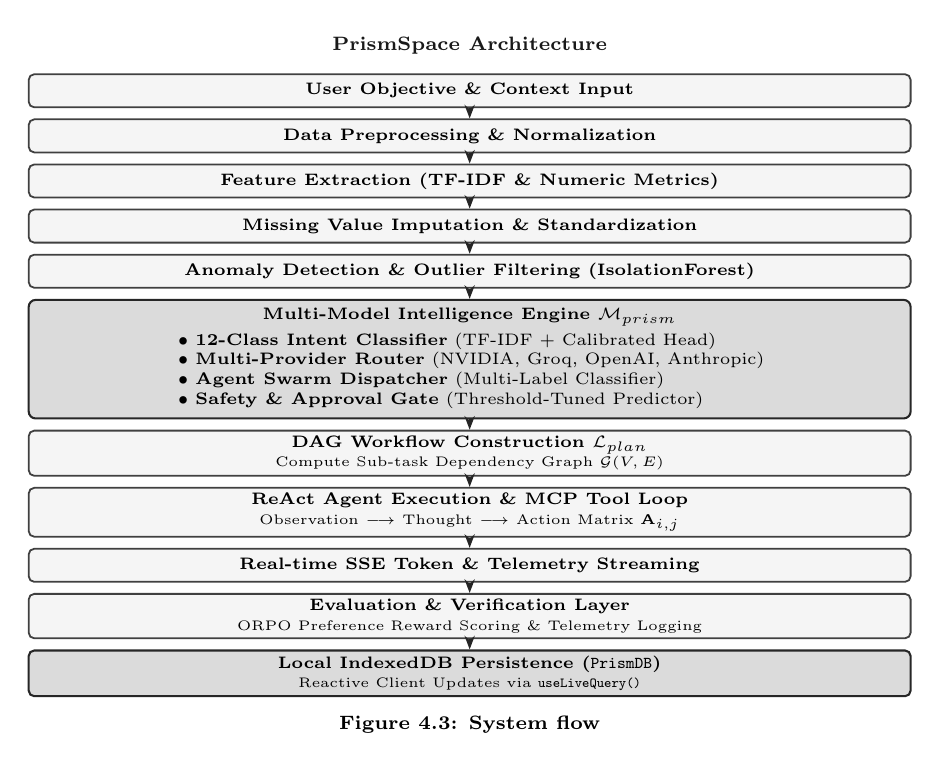
\begin{tikzpicture}[
    x=1cm, y=1cm,
    font=\sffamily,
    node distance=0.13cm,
    box/.style={
        rectangle,
        draw=black!75,
        line width=0.65pt,
        fill=black!4,
        rounded corners=2pt,
        minimum width=11.2cm,
        minimum height=0.42cm,
        inner ysep=2.0pt,
        inner xsep=3pt,
        align=center,
        font=\fontsize{6.3}{7.5}\selectfont
    },
    enginebox/.style={
        rectangle,
        draw=black!85,
        line width=0.75pt,
        fill=black!14,
        rounded corners=2.5pt,
        minimum width=11.2cm,
        inner ysep=3.0pt,
        inner xsep=4pt,
        align=center,
        font=\fontsize{5.9}{7.1}\selectfont
    },
    shadedbox/.style={
        rectangle,
        draw=black!85,
        line width=0.75pt,
        fill=black!14,
        rounded corners=2pt,
        minimum width=11.2cm,
        minimum height=0.44cm,
        inner ysep=2.0pt,
        inner xsep=3pt,
        align=center,
        font=\fontsize{6.3}{7.5}\selectfont
    },
    arrow/.style={
        -{Stealth[scale=0.8]},
        line width=0.7pt,
        draw=black!85
    }
]

    % Header text matching diagram
    \node[font=\bfseries\fontsize{7.5}{9.0}\selectfont, text=black!90] (arch_title) at (0, 0) {PrismSpace Architecture};

    % 1. User Objective
    \node[box, below=0.12cm of arch_title] (b1) {\textbf{User Objective \& Context Input}};

    % 2. Preprocessing
    \node[box, below=of b1] (b2) {\textbf{Data Preprocessing \& Normalization}};

    % 3. Feature Extraction
    \node[box, below=of b2] (b3) {\textbf{Feature Extraction (TF-IDF \& Numeric Metrics)}};

    % 4. Imputation
    \node[box, below=of b3] (b4) {\textbf{Missing Value Imputation \& Standardization}};

    % 5. Anomaly Detection
    \node[box, below=of b4] (b5) {\textbf{Anomaly Detection \& Outlier Filtering (IsolationForest)}};

    % 6. Engine
    \node[enginebox, below=of b5] (b6) {
        \textbf{Multi-Model Intelligence Engine $\mathcal{M}_{\text{prism}}$}\\[0.14em]
        \begin{tabular}{@{\hspace{0.25cm}}l}
        $\bullet$ \textbf{12-Class Intent Classifier} (TF-IDF + Calibrated Head)\\
        $\bullet$ \textbf{Multi-Provider Router} (NVIDIA, Groq, OpenAI, Anthropic)\\
        $\bullet$ \textbf{Agent Swarm Dispatcher} (Multi-Label Classifier)\\
        $\bullet$ \textbf{Safety \& Approval Gate} (Threshold-Tuned Predictor)
        \end{tabular}
    };

    % 7. DAG Workflow
    \node[box, below=of b6] (b7) {
        \textbf{DAG Workflow Construction $\mathcal{L}_{\text{plan}}$}\\[-0.08em]
        {\fontsize{5.2}{6.2}\selectfont Compute Sub-task Dependency Graph $\mathcal{G}(V, E)$}
    };

    % 8. ReAct Agent
    \node[box, below=of b7] (b8) {
        \textbf{ReAct Agent Execution \& MCP Tool Loop}\\[-0.08em]
        {\fontsize{5.2}{6.2}\selectfont Observation $\longrightarrow$ Thought $\longrightarrow$ Action Matrix $\mathbf{A}_{i,j}$}
    };

    % 9. Real-time SSE
    \node[box, below=of b8] (b9) {\textbf{Real-time SSE Token \& Telemetry Streaming}};

    % 10. Evaluation
    \node[box, below=of b9] (b10) {
        \textbf{Evaluation \& Verification Layer}\\[-0.08em]
        {\fontsize{5.2}{6.2}\selectfont ORPO Preference Reward Scoring \& Telemetry Logging}
    };

    % 11. Persistence
    \node[shadedbox, below=of b10] (b11) {
        \textbf{Local IndexedDB Persistence (\texttt{PrismDB})}\\[-0.08em]
        {\fontsize{5.2}{6.2}\selectfont Reactive Client Updates via \texttt{useLiveQuery()}}
    };

    % Caption
    \node[font=\bfseries\fontsize{7.2}{8.5}\selectfont, below=0.12cm of b11] (caption) {Figure 4.3: System flow};

    % Arrows
    \draw[arrow] (b1) -- (b2);
    \draw[arrow] (b2) -- (b3);
    \draw[arrow] (b3) -- (b4);
    \draw[arrow] (b4) -- (b5);
    \draw[arrow] (b5) -- (b6);
    \draw[arrow] (b6) -- (b7);
    \draw[arrow] (b7) -- (b8);
    \draw[arrow] (b8) -- (b9);
    \draw[arrow] (b9) -- (b10);
    \draw[arrow] (b10) -- (b11);

\end{tikzpicture}%
}
\end{frame}
\end{document}
